\chapter{Marco te\'orico.}

\section{Teor\'ia de interpolaci\'on.}

\hspace{0.4cm} En el subcampo matem\'atico del an\'alisis num\'erico, se denomina interpolaci\'on a la obtenci\'on de nuevos puntos partiendo del conocimiento de un conjunto discreto de puntos.


\hspace{0.4cm} En ciertos casos el usuario conoce el valor de una funci\'on $f(x)$ en una serie de puntos $x_{1}, x_{2},..., x_{N}$, pero no se conoce una 
expresi\'on anal\'itica de $f(x)$ que permita calcular el valor de la funci\'on para un punto arbitrario. Un ejemplo claro son las mediciones de laboratorio, donde se mide cada minuto un valor, pero se requiere el valor en otro punto que no ha sido medido. Otro ejemplo son mediciones de temperatura en la superficie
de la Tierra, que se realizan en equipos o estaciones meteorol\'ogicas y se necesita calcular la temperatura en un punto cercano, pero distinto al punto de medida.

\hspace{0.4cm} La idea de la interpolaci\'on es poder estimar $f(x)$ para un valor de x arbitrario, a partir de la construcci\'on de una curva o superficie que une los puntos donde se han realizado las mediciones y cuyo valor si se conoce. Se asume que el punto arbitrario x se encuentra dentro de los l\'imites de los puntos de medici\'on, en caso contrario se llamar\'ia extrapolaci\'on. 

\hspace{0.4cm} Un proceso de interpolaci\'on se realiza en dos etapas:

\begin{itemize}
  \item Hacer un ajuste de los datos disponibles con una funci\'on interpolante.
  \item Evaluar la funci\'on interpolante en el punto de inter\'es x.
\end{itemize}


\hspace{0.4cm} Este proceso en dos etapas no es necesariamente el m\'as 
eficiente. La mayor\'ia de algoritmos comienzan con un punto cercano $f(x_{i})$, y poco a poco van aplicando correcciones m\'as pequenas a medida que la 
informaci\'on de valores $f(xi)$ m\'as distantes son incorporadas. El procedimiento toma aproximadamente $O(N^{2})$ operaciones. Si la funci\'on tiene un comportamiento suave, la \'ultima correci\'on ser\'a la m\'as pequena y puede ser utilizada para estimar un l\'imite a rango de error.


\hspace{0.4cm} Dentro de las intepolaciones m\'as usadas podemos destacar,

\begin{itemize}
  \item Interpolaci\'on lineal
  \item Interpolaci\'on de Hermite
  \item Interpolaci\'on polin\'omica 
  \item Interpolaci\'on de Splines 

\end{itemize}

\subsection{Interpolaci\'on lineal.\\}

\hspace{0.4cm} La interpolaci\'on lineal es un procedimiento muy utilizado para estimar los valores que toma una funci\'on en un intervalo del cual conocemos sus valores en los extremos $(x_{1}, f(x_{1}))$ y $(x_{2},f(x_{2}))$. Para estimar este valor utilizamos la aproximaci\'on a la funci\'on f(x) por medio de una recta $r(x)$ (de ah\'i el nombre de interpolaci\'on lineal, ya que tambi\'en existe la interpolaci\'on cuadr\'atica). 


\hspace{0.4cm} La expresi\'on de la interpolaci\'on lineal se obtiene del polinomio interpolador de Newton de grado uno. Aunque s\'olo existe un \'unico polinomio que interpola una serie de puntos, existen diferentes formas de calcularlo. Este m\'etodo es \'util para situaciones que requieran un n\'umero bajo de puntos para interpolar, ya que a medida que crece el n\'umero de puntos, tambi\'en lo hace el grado del polinomio.

\hspace{0.4cm} Existen ciertas ventajas en el uso de este polinomio respecto al polinomio interpolador de Lagrange. Por ejemplo, si fuese necesario a\~nadir alg\'un nuevo punto o nodo a la funci\'on, tan s\'olo habr\'ia que calcular este \'ultimo punto, dada la relaci\'on de recurrencia existente y demostrada anteriormente.

\hspace{0.4cm}El primer paso para hallar la f\'ormula de la interpolaci\'on es definir la pendiente de orden n de manera recursiva, as\'i,

\begin{itemize}
  \item $f_{0}(x_{i})$ es el t\'ermino i-\'esimo de la secuencia. 
  \item $\displaystyle{f_{1}(x_{0},x_{1}) = \frac{f_{0}(x_{1})-f_{0}(x_{0})}{x_{1}-x_{0}}}$
  \item $\displaystyle{f_{2}(x_{0},x_{1},x_{2}) = \frac{f_{1}(x_{1},x_{2})-f_{1}(x_{0},x_{1})}{x_{2}-x_{0}}}$
\end{itemize}

\hspace{0.4cm} En general,

\begin{center}
$\displaystyle{f_{i}(x_{0},x_{1},...,x_{i-1},x_{i}) = \frac{f_{i-1}(x_{1},...,x_{i-1},x_{i})-f_{i-1}(x_{0},x_{1},...,x_{i-1} )}{x_{i}-x_{0}}}$
\end{center}


\noindent donde  $\displaystyle{x_{i}-x_{j}}$ representa la distancia entre dos elementos.

\hspace{0.4cm} Puede apreciarse c\'omo en la definici\'on general se usa la pendiente del paso anterior, $f_{i-1}(x_{1},...,x_{i-1},x_{i})$, a la cual se le resta la pendiente previa de mismo orden, es decir, el sub\'indice de los t\'erminos se decrementa en 1, como si se desplazara, para obtener $f_{i-1}(x_{0},x_{1},...,x_{i-1})$.

\hspace{0.4cm} N\'otese tambi\'en que aunque el t\'ermino inicial siempre es $x_{0}$ este puede ser en realidad cualquier otro, por ejemplo, se puede definir $f_{1}(x_{i-1},x_{i})$ de manera an\'aloga al caso mostrado arriba.

\hspace{0.4cm} Una vez conocemos la pendiente, ya es posible definir el polinomio de grado n de manera tambi\'en recursiva, as\'i,

\begin{itemize}
  \item $p_{0}(x) = f_{0} (x_{0}) =x_{0}$.  Se define as\'i ya que este valor es el \'unico que se ajusta a la secuencia original para el primer t\'ermino. 
  \item $\displaystyle{p_{1}(x) = p_{0}(x) +  f_{1} (x_{0},x_{1}) (x-x_{0})}$.
  \item $\displaystyle{p_{2}(x) = p_{1}(x) +  f_{2} (x_{0},x_{1},x_{2}) (x-x_{0})(x-x_{1})}$.
\end{itemize}

\hspace{0.4cm} En general,

\begin{center}
$\displaystyle{p_{i}(x) = p_{i-1}(x) +  f_{i} (x_{0},x_{1},...,x_{i-1},x_{i}) \prod_{j=0}^{i-1}(x-x_{j})}$
\end{center}


\subsection{Interpolaci\'on de Lagrange.\\}

\hspace{0.4cm} Empezamos con un conjunto de $n+1$ puntos en el plano (que tengan diferentes coordenadas x), $(x_{0}, y_{0}), (x_{1}, y_{1}), (x_{2}, y_{2}),...,(x_{n}, y_{n})$. As\'i, queremos encontrar una funci\'on polin\'omica que pase por esos $n+1$ puntos y que tengan el menor grado posible. Un polinomio que pase por varios puntos determinados se llama un polinomio de interpolaci\'on.

\hspace{0.4cm} Una posible soluci\'on viene dada por el  polinomio de interpolaci\'on de Lagrange. Lagrange public\'o su f\'ormula en 1795 pero ya hab\'ia sido publicada en 1779 por Waring y redescubierta por Euler en 1783.

\hspace{0.4cm} Dado un conjunto de $k + 1$ puntos $(x_{0}.x_{1}),...,(x_{k}.x_{k+1})$, donde todos los $x_{j}$ se asumen distintos, el polinomio interpolador en la forma de Lagrange es la combinaci\'on lineal,

\begin{center}
$\displaystyle{L(x) = \sum_{j=0}^{k} y_{j} l_{j}(x)}$
\end{center}


\noindent donde $ l_{j}(x)$ son las bases polin\'omicas de Lagrange ,

\begin{center}
$\displaystyle{l_{j}(x) = \prod_{i=0,i \neq j}^{k} \frac{x-x_{i}}{x_{j}-x_{i}}  }$
\end{center}

\hspace{0.4cm} La funci\'on que estamos buscando es una funci\'on polin\'omica $L(x)$ de grado $k$ con el problema de interpolaci\'on puede tener tan solo una soluci\'on, pues la diferencia entre dos tales soluciones, ser\'ia otro polinomio de grado $k$ a lo sumo, con $k+1$ ceros. Por lo tanto, $L(x)$ es el \'unico polinomio interpolador.


\hspace{0.4cm} Si se aumenta el n\'umero de puntos a interpolar (o nodos) con la intenci\'on de mejorar la aproximaci\'on a una funci\'on, tambi\'en lo hace el grado del polinomio interpolador as\'i obtenido, por norma general. De este modo, aumenta la dificultad en el c\'alculo, haci\'endolo poco operativo manualmente a partir del grado 4, dado que no existen m\'etodos directos de resoluci\'on de ecuaciones de grado 4, salvo que se puedan tratar como ecuaciones bicuadradas, situaci\'on extremadamente rara.

\hspace{0.4cm} La tecnolog\'ia actual permite manejar polinomios de grados superiores sin grandes problemas, a costa de un elevado consumo de tiempo de computaci\'on. Pero, a medida que crece el grado, mayores son las oscilaciones entre puntos consecutivos o nodos. Se podr\'ia decir que a partir del grado 6 las oscilaciones son tal que el m\'etodo deja de ser v\'alido, aunque no para todos los casos.

\hspace{0.4cm} Sin embargo, pocos estudios requieren la interpolaci\'on de tan s\'olo 6 puntos. Se suelen contar por decenas e incluso centenas. En estos casos, el grado de este polimonio ser\'ia tan alto que resultar\'ia inoperable. Por lo tanto, en estos casos, se recurre a otra t\'ecnica de interpolaci\'on, como por ejemplo a la Interpolaci\'on polin\'omica de Hermite o a los splines c\'ubicos. Otra gran desventaja, respecto a otros m\'etodos de interpolaci\'on, es la necesidad de recalcular todo el polinomio si se var\'ia el n\'umero de nodos.

\hspace{0.4cm} Aunque el polinomio interpolador de Lagrange se emplea mayormente para interpolar funciones e implementar esto f\'acilmente en una computadora, tambi\'en tiene otras aplicaciones en el campo del \'algebra exacta, lo que ha hecho m\'as c\'elebre a este polinomio, por ejemplo en el campo de los proyectores ortogonales.


\subsection{Interpolaci\'on de Hermite.\\}

\hspace{0.4cm} El objetivo de esta interpolaci\'on Hermite es minimizar el error producido en la interpolaci\'on de Lagrange de la funci\'on $f(x)$ sobre el intervalo $[a, b]$ sin aumentar el grado del polinomio interpolador.


\hspace{0.4cm} Dados un entero no negativo N y  N + 1 puntos $(x_{0},..., x_{N})$ de la recta distintos dos a dos y los valores $f^{(j)} (x_{i})$, donde $0<i<N$ y $0<j<k_{i-1}$ de una funci\'on f y de sus derivadas, encontrar un polinomio de grado $m = (k_{0} +k_{1} +...+k_{n-1},)$ tal que,

\begin{center}
$\displaystyle{P^{(j)} (x_{i}) = f^{(j)} (x_{i}), para \hspace{0.2cm} 0<i<N \hspace{0.2cm}y \hspace{0.2cm} 0<j<k_{i-1}}$
\end{center}

\hspace{0.4cm} El problema de interpolaci\'on de Hermite tiene soluci\'on \'unica, que se llama polinomio interpolador de Hermite. En lugar de interpolar sobre un soporte de puntos (de Tchebycheff) donde en general se desconoce el valor de la funci\'on, de hace de otra manera, imponiendo unas condiciones al polinomio,

\begin{itemize}
  \item  Igualar el valor de la funci\'on en en los puntos del soporte, $P (x_{i}) = f^{(j)}$
  \item Igualar el valor de algunas derivadas de la funci\'on tambi\'en en los puntos del soporte, $P^{(j)} (x_{i}) = f^{(j)} (x_{i})$
\end{itemize}

\hspace{0.4cm} Por lo que podemos dejar el polinomio de Hermite de grado (n-1) expresado de la siguiente manera,

\begin{center}
$\displaystyle{L(x) = \sum_{j=0}^{k} y_{j} l_{j} (x) }$
\end{center}

\noindent donde $l_{j}(x)$ son los polinomios de la base de Lagrange.


\subsection{Interpolaci\'on Polin\'omica.\\}

\hspace{0.4cm}Asumamos que se tiene una tabla con n puntos, $(x_{1},y_{1})...,(x_{n},y_{n})$, donde los valores $x_{i}$, para $i=1,...,n$ est\'an ordenados de forma creciente y todos ellos son distintos. Supongamos que dichos puntos se representan en un plano cartesiano y se quiere determinar una curva suave que interpole dichos valores. As\'i, se desea determinar una curva que est\'e definida para todos los $x$ y tome los valores correspondientes de $y$, esto es, que interpole todos los datos de la tabla. Cabe destacar que los puntos considerados se les conoce como nodos.


\vspace{0.5cm}

\hspace{0.4cm} La primera idea natural es usar una funci\'on polinomial que represente esta curva, la cual se puede representar como sigue,

\vspace{0.5cm}
\begin{center}

$\displaystyle{P_{n} = \sum_{i=0}^{n-1} a_{i}x^{i}}$

\end{center}

\noindent tal curva se le conoce como funci\'on polinomial interpoladora de grado n. N\'otese que en cada nodo se satisface que $P_{n}(x_{k})=y_{k}$, donde $k=1,...,n$.

\vspace{0.5cm}

\hspace{0.4cm} As\'i, se tiene que si la tabla es representada mediante una funci\'on subyacente $f(x)$ tal que $f(x_{k})=y_{k}$, para todo k, entonces esta funci\'on puede ser aproximada mediante $P_{n}$, en los puntos intermedios.


\vspace{0.5cm}

\hspace{0.4cm} No ser\'ia descabellado pensar que a medida que los nodos se incrementan, la aproximaci\'on ser\'ia cada vez mejor, lamentablemente esto no siempre es cierto, debido a que en el caso de tener una data con mucho ruido la interpolaci\'on no tendr\'ia mucho sentido ya que la varianza de los valores interpolados ser\'ia muy grande. En este caso, los polinomios interpoladores resultantes ser\'ian una mala representaci\'on de la funci\'on subyacente.

\vspace{0.5cm}

\hspace{0.4cm} Para evitar este fen\'omeno, puede ser de utilidad relajar la condici\'on de que $f(x)$ deber\'ia ser una funci\'on que interpole todos los valores dados y en su lugar usar un trozo de un polinomio local de interpolaci\'on. La funci\'on mediante la cual se logra esta interpolaci\'on se le conoce como spline.


\section{Splines.}

\vspace{1 cm}

\hspace{0.4cm} Una funci\'on spline $S(x)$ es una funci\'on que consta de trozos de polinomios unidos por ciertas condiciones de suavizado. Un ejemplo simple, es una funci\'on poligonal (spline de primer grado), la cual se forma por polinomios lineales unidos, los cuales se definen entre cada par de nodos. Entre los nodos $x_{j}$ y $x_{j+1}$ se define un spline de primer grado como sigue, \\

\begin{center}

$\displaystyle{S(x) = a_{j}x + b_{j} = S_{j}(x)}$

\end{center}

\vspace{0.5cm}

\noindent este spline es lineal. Usualmente $S(x)$ se define como $S_{1}(x)$ para $x<x_{1}$ y como $S_{n-1}(x)$ para $x>x_{n}$, donde $x_{1}$ y $x_{n}$ son nodos frontera (ver figura \ref{spline_l}).


\begin{figure}[h]
  \scalebox{0.50}{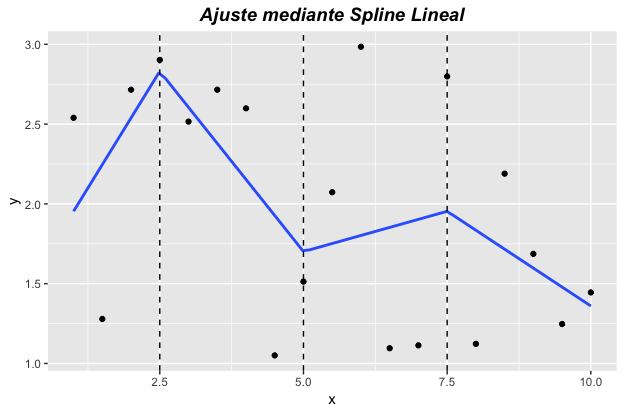
\includegraphics{images/spline_lineal.png}}
\caption{Spline Lineal.}
\label{spline_l}
\end{figure}




\vspace{0.5cm}

\hspace{0.4cm} Un spline de segundo grado es una uni\'on de polinomios cuadr\'aticos tal que $S(x)$ y su derivada $S^{(1)}(x)$ son continuas (ver figura \ref{spline_c}). Los polinomios $P(x)$ a trav\'es de los que construimos el Spline tienen grado 2. Esto quiere decir, que va a tener la forma $P(x) = ax^2 + bx + c$.

\hspace{0.4cm} Como en la interpolaci\'on segmentaria lineal, vamos a tener $N-1$ ecuaciones (donde N son los puntos sobre los que se define la funci\'on). La interpolaci\'on cuadr\'atica nos va a asegurar que la funci\'on que nosotros generemos a trozos con los distintos $P(x)$ va a ser continua, ya que para sacar las condiciones que ajusten el polinomio, vamos a determinar como condiciones,

\begin{itemize}
  \item Que las partes de la funci\'on a trozos P(x) pasen por ese punto. Es decir, que las dos Pn(x) que rodean al f(x) que queremos aproximar, sean igual a f(x) en cada uno de estos puntos.
  \item Que la derivada en un punto siempre coincida para ambos "lados" de la funci\'on definida a trozos que pasa por tal punto com\'un.
  \item Esto sin embargo no es suficiente, y necesitamos una condici\'on m\'as, la cual se obtiene a partir de una condici\'on de borde.
\end{itemize}




\hspace{0.4cm} Por su parte un spline c\'ubico, se representa mediante la uni\'on de polinomios c\'ubicos con primera y segunda derivada continuas (ver figura \ref{spline_3}). Este spline debido a su flexibilidad es el m\'as usado en las aplicaciones.

\vspace{0.5cm}

\begin{figure}[h]
  \scalebox{0.50}{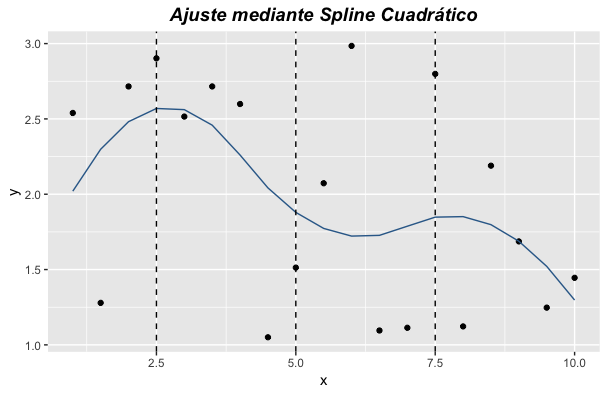
\includegraphics{images/spline_cuadratico.png}}
\caption{Spline Cuadr\'atico.}
\label{spline_c}
\end{figure}


\hspace{0.4cm}Formalmente un spline c\'ubico con nodos $x_{1},...x_{n}$ se define a partir de un conjunto de polinomios de la forma,\\

\begin{center}

$\displaystyle{S_{j}(x) = a_{j} + b_{j}x +c_{j}x^2 +d_{j}x^3}$
\end{center}


\vspace{0.5cm}

\noindent con $x_{j}<x<x_{j+1}$, sujeto a las siguientes condiciones,\\


\begin{center}

$\displaystyle{a_{j-1} + b_{j-1}x_{j} +c_{j-1}x_{j}^2 +d_{j-1}x_{j}^3 = a_{j} + b_{j}x_{j} +c_{j}x_{j}^2 +d_{j}x_{j}^3}$\\
$\displaystyle{ b_{j-1} +2c_{j-1}x_{j} +3d_{j-1}x_{j}^2 = b_{j} +2c_{j}x_{j} +3d_{j}x_{j}^2}$\\
$\displaystyle{ 2c_{j-1} +6d_{j-1}x_{j} = 2c_{j} +6d_{j}x_{j}}$\\
$\displaystyle{ c_{0} = d_{0} = c_{n} =d_{n}}$

\end{center}

\begin{figure}[h]
  \scalebox{0.50}{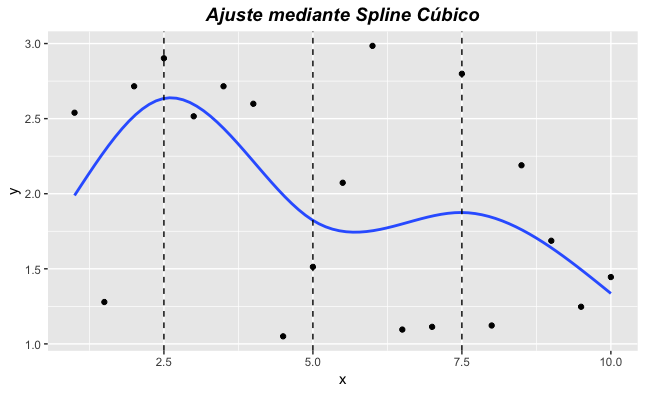
\includegraphics{images/spline_cubico.png}}
\caption{Spline C\'ubico.}
\label{spline_3}
\end{figure}


\hspace{0.4cm}As\'i para n nodos, existen $4(n-1)$ variables y $4(n-1)-2$ restricciones. Las mismas se deben a la necesidad de que el spline c\'ubico sea igual en los valores dados en cada nodo. Las primeras tres restricciones aseguran que la funci\'on resultante en su primera y segunda derivada sean continuas en los nodos. La restricci\'on final significa que el spline c\'ubico es lineal en el punto inicial y final de la muestra. Sin embargo, es importante resaltar que el spline c\'ubico tiene tercera derivada discontinua en los nodos.

\hspace{0.4cm}Debido a que hacen falta dos restricciones de borde, estas se deben a\~nadir. As\'i  $S^{(2)}(x_{1}) = S^{(2)}(x_{n}) = 0$ son las restricciones faltantes, estan hacen referencia a que el spline sea un spline c\'ubico natural. Como se mencion\'o al inicio si se considera una interpolaci\'on polinomial global de un conjunto de datos con mucho ruido pueden surgir aproximaciones no deseables e inestables. En constrate, un spline c\'ubico de interpolaci\'on encaja perfectamente con la suavidad de la funci\'on subyacente.

\begin{figure}[h]
  \scalebox{0.50}{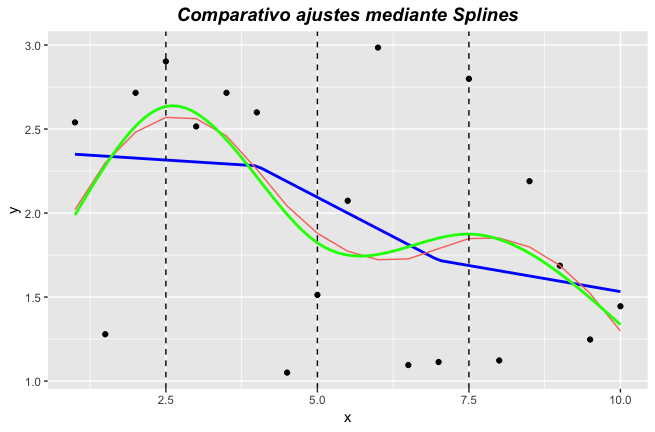
\includegraphics{images/Comparativo_splines.png}}
\caption{Comparativo Splines.}
\end{figure}

\vspace{0.5cm}

\hspace{0.4cm} Otra caracter\'istica de los splines es que con la adici\'on de un par\'ametro s\'olo se aumenta la dimensionalidad del espacio de par\'ametros en una unidad, ya que tres de los cuatro par\'ametros est\'an restringidos. De igual forma, al incrementar el n\'umero de nodos los splines toman formas funcionales m\'as flexibles, lo cual muestra la relaci\'on entre el grado aproximaci\'on que se logra con el spline y el n\'umero de nodos que lo definen.

\vspace{0.5cm}

\hspace{0.4cm} Mientras que las funciones spline son una herramienta interesante para interpolar funciones suaves, encontrarlas num\'ericamente no es tarea f\'acil. Una manera eficiente y muy estable para generar los splines necesarios para aproximar la funci\'on subyacente $f(x)$, es usando las bases de los B-splines c\'ubicos.

\vspace{0.5cm}

\subsection{Bases de splines.\\}

\hspace{0.4cm} En el subcampo matem\'atico de an\'alisis num\'erico, una B-spline o Basis spline (o traducido una l\'inea polin\'omica suave b\'asica), es una funci\'on spline que tiene el m\'inimo soporte con respecto a un determinado grado, suavidad y partici\'on del dominio. Un teorema fundamental establece que cada funci\'on spline de un determinado grado, suavidad y partici\'on del dominio, se puede representar como una combinaci\'on lineal de B-splines del mismo grado y suavidad, y sobre la misma partici\'on. El t\'ermino B-spline fue propuesto por Isaac Jacob Schoenberg y es la abreviatura de spline b\'asica. Las B-splines pueden ser evaluadas de una manera num\'ericamente estable por el algoritmo de Boor. De un modo simplificado, se han creado variantes potencialmente m\'as r\'apidas que el algoritmo de Boor, pero adolecen comparativamente de una menor estabilidad.

\hspace{0.4cm} En el subcampo de la inform\'atica de dise\~no asistido por computadora y de gr\'aficos por computadora, el t\'ermino B-spline se refiere con frecuencia a una curva parametrizada por otras funciones spline, que se expresan como combinaciones lineales de B-splines (en el sentido matem\'atico anterior). Una B-spline es simplemente una generalizaci\'on de una curva de B\'ezier, que puede evitar el fen\'omeno Runge sin necesidad de aumentar el grado de la B-spline. Este fen\'omeno, se presenta al realizar interpolaci\'on lineal usando nodos equidistantes, b\'asicamente es un problema que se presenta con el error de aproximaci\'n en los extremos del intervalo que se este considerando, as\'i a medida que crece el n\'umero de nodos el error de aproximaci\'on se incrementa. 


\hspace{0.4cm} Supongamos que tenemos un conjunto infinito de nodos $...<x_{-2}<x_{-1}<x_{0}<x_{1}<x_{2}<...$, entonces el j-\'esimo B-spline de grado cero es igual a $B^{0}_{j}(x)=1$, si $x_{j} \leq x \leq x_{j+1}$ y $B^{0}_{j}(x)=0$ en otro caso. Con la funci\'on $B^{0}_{j}(x)$ como punto de partida se puede generar B-splines de grados mayores mediante la siguiente f\'ormula recursiva,\\

\begin{center}

$\displaystyle{B^{k}_{j}(x) = \frac{(x-x_{j})B^{k-1}_{j}(x)}{x_{j+k}-x_{j}} + \frac{(x_{j+k+1}-x)B^{k-1}_{j+1}(x)}{x_{j+k+1}-x_{j+1}}}$
\end{center}

\vspace{0.5cm}

\noindent para $k\geq 1$. As\'i un B-spline de grado $k$ se define como,\\

\begin{center}

$\displaystyle{S^{k}(x) = \sum_{j=-\infty}^{\infty} \theta^{k}_{j} B^{k}_{j-k}(x)}$
\end{center}

\vspace{0.5cm}

\hspace{0.4cm} Los coeficientes $\theta^{k}_{j}$ se llaman puntos de control o puntos de Boor. Hay $m-(n+1)$ puntos de control que forman una envoltura convexa.. Una buena interrogante ser\'ia el como se determina el valor de estos coeficientes en la expresi\'on anterior. Note que los B-splines de grado positivo no son ortogonales y por ende no poseen una expresi\'on simple para sus coeficientes.


Sin embargo, los c\'alculos empleados para los B-splines interpoladores de grado cero y uno, son bastante sencillos,\\

\begin{center}

$\displaystyle{S^{0}(x) = \sum_{j=-\infty}^{\infty} y_{j} B^{0}_{j}(x),\hspace{0.4cm} S^{1}(x) = \sum_{j=-\infty}^{\infty} y_{j} B^{1}_{j-1}(x) }$
\end{center}

\vspace{0.5cm}


\hspace{0.4cm} Cuando los nodos son equidistantes, la B-spline se dice que es uniforme, de otro modo ser\'a no uniforme. Si dos nodos tj son id\'enticos, cualquiera de las posibles formas indeterminadas 0/0 se consideran 0.


\subsection{B-spline uniforme.\\}

\hspace{0.4cm} Cuando la B-spline es uniforme, las B-splines b\'asicas para un determinado grado n son s\'olo copias cambiadas de una a otra. Una alternativa no recursiva de la definici\'on de la B-splines $m-n+1$ b\'asica es,


\begin{center}
$\displaystyle{B_{j}^{n}(t)= B_{n}(t-t_{j}), \hspace{0.2cm}para \hspace{0.2cm}j=0,...,m-n-1 }$
\end{center}

\noindent con,

\begin{center}
$\displaystyle{B_{n}(t):= \frac{n+1}{n} \sum_{i=0}^{n+1}w_{i}^{n}(t - t_{i})_{+}^{n}   }$
\end{center}


\noindent donde,

\begin{center}
$\displaystyle{w_{i}^{n} := \prod_{j=0, j\neq i}^{n+1} \frac{1}{t_{j}- t_{i}}}$
\end{center}

\noindent n\'otese que $(t - t_{i})_{+}^{n}$ es la funci\'on potencia truncada definida como,

$$ (t - t_{i})_{+}^{n} := \left\{ % para la llave grandota
        \begin{tabular}{cc}
        	$0$ & si $t < t_{i}$ \\
        	$(t - t_{i})^{n}$ & si $t \ge t_{i}$ \\
        \end{tabular}
\right. $$


\subsection{B-spline cardinal.\\}

\hspace{0.4cm} Si se define $B_{0}$ como la funci\'on caracter\'istica de ${\displaystyle [-{\tfrac {1}{2}},{\tfrac {1}{2}}]}$, y $B_{k}$ recursivamente como el producto convoluci\'on,


\begin{center}
$\displaystyle{B_{k} := B_{k-1}*B_{0}, \hspace{0.2cm} k=1,2,... }$
\end{center}

\noindent entonces $B_{k}$ se llaman B-splines cardinales (centradas). Esta definici\'on se remonta a Schoenberg. $B_{k}$ tiene soporte compacto ${\displaystyle [-{\tfrac {k+1}{2}},{\tfrac {k+1}{2}}]}$ y es una funci\'on impar. Como ${\displaystyle k\rightarrow \infty }$ las B-splines cardinales normalizadas tienden a la funci\'on de Gauss.

\hspace{0.4cm} Cuando el n\'umero de puntos de control de Boor es el mismo que el grado, la B-Spline degenera en una curva de B\'ezier. La forma de las funciones base es determinada por la posici\'on de los nodos. Escalar o trasladar el vector de nodo no altera las funciones de base.

\hspace{0.4cm} El spline est\'a contenido en el casco convexo de sus puntos de control. Una B-spline b\'asica de grado n $B_{i}^{n}(t)$ es distinta de cero s\'olo en el intervalo $[t_{i}, t_{i+n+1}]$ esto es,

$$ B_{i}^{n}(t) = \left\{ % para la llave grandota
        \begin{tabular}{cc}
        	$ > 0$ & si $t_{i}  \leq  t < t_{i+n+1}$ \\
        	$0$ & si $resto$ \\
        \end{tabular}
\right. $$

\hspace{0.4cm} En otras palabras si manipulamos un punto de control cambiamos s\'olo el comportamiento local de la curva y no el comportamiento global como con las curvas de B\'ezier. La funci\'on base se pueda obtener del polinomio de Bernstein. Algunos ejemplos de las bases B-splines se muestran acontinuaci\'on,

\subsection{B-spline constante.\\}

\hspace{0.4cm} La B-spline constante es la spline m\'as simple. Se define en un solo tramo de nodo y ni siquiera es continua en los nodos. Es s\'olo la funci\'on indicador de los diferentes tramos de nodo.

$$ B_{j}^{0}(t) = 1_{[t_{j},t_{j+1})} = \left\{ % para la llave grandota
        \begin{tabular}{cc}
        	$ 1$ & si $t_{j}  \leq  t < t_{j+1}$ \\
        	$0$ & si $resto$ \\
        \end{tabular}
\right. $$



\subsection{B-spline lineal.\\}

\hspace{0.4cm} La B-spline lineal se define en dos tramos de nodo consecutivos y es continua sobre los nodos, pero no diferenciable.

$$ B_{j}^{1}(t) = \left\{ % para la llave grandota
        \begin{tabular}{cc}
        	$\frac{t-t_{j}}{t_{j+1}-t_{j}} $ & si $t_{j}  \leq  t < t_{j+1}$ \\
        	$\frac{t_{j+2}-t}{t_{j+2}-t_{j+1}} $ & si $t_{j+1}  \leq  t < t_{j+2}$ \\
        	$0$ & si $resto$ \\
        \end{tabular}
\right. $$


\subsection{B-spline cuadr\'atica uniforme.\\}

\hspace{0.4cm} Las B-splines cuadr\'aticas con nodo-vector uniforme es una forma com\'un de B-spline. La funci\'on base puede ser calculada f\'acilmente , y es igual para cada segmento, en este caso.

$$ B_{j}^{2}(t) = \left\{ % para la llave grandota
        \begin{tabular}{cc}
        	$\frac{1}{2} (1-t)^2$ \\
        	$-t^2+t+\frac{1}{2}$ \\
        	$\frac{1}{2} t^2$ \\
        \end{tabular}
\right. $$

\hspace{0.4cm} Escrito en forma de matriz, esto es,


\begin{center}
$\displaystyle{S_{i}(t) = \begin{bmatrix} t^2 & t & 1  \end{bmatrix} \frac{1}{2} \begin{bmatrix} 1 & -2 & 1\\ -2 & 2 & 0  \\ 1 & 1 & 0 \end{bmatrix} \begin{bmatrix}  \theta_{i-1} \\ \theta_{i} \\ \theta_{i+1}  \end{bmatrix} , \hspace{0.2cm} para \hspace{0.2cm} t \in [0,1],\hspace{0.2cm}  i=1,2,...,m-1 }$
\end{center}


\subsection{B-spline c\'ubica.\\}

\hspace{0.4cm} Una formulaci\'on B-spline para un solo segmento puede ser escrita como,

\begin{center}
$\displaystyle{S_{i}(t) = \sum_{k=0}^{3} \theta_{i-3+k} B_{i-3+k}^{3}(t) \hspace{0.2cm} con \hspace{0.2cm} t \in [0,1]  }$
\end{center}


\noindent donde $S_{i}$ es el i-\'esimo segmento B-spline, $\theta$ es el conjunto de puntos de control, el segmento i y k es el \'indice del punto de control local y $ B_{i-3+k}^{3}(t)$ representa la base de B-spline de grado 3. Un conjunto de puntos de control $\theta$ ser\'ia  ${\displaystyle \theta_{i}^{w}=(w_{i}x_{i},w_{i}y_{i},w_{i}z_{i},w_{i})}$ donde el ${\displaystyle w_{i}}$ es el peso, tirando de la curva hacia el punto de control ${\displaystyle \theta_{i}}$ mientras que aumenta o se desplazan fuera de la curva, a la vez que disminuye.


\hspace{0.4cm} Toda una serie de segmentos se definir\'ia como,

\begin{center}
$\displaystyle{S(t) = \sum_{i=0}^{m-1} \theta_{i} B_{i}^{3}(t)  }$
\end{center}

\noindent donde i es el n\'umero de puntos de control y t es un par\'ametro global dados los valores de los nodos. Esta formulaci\'on expresa una curva B-spline como una combinaci\'on lineal de funciones B-spline b\'asicas, de ah\'i el nombre.

\hspace{0.4cm} Hay dos tipos de B-spline - uniforme y no uniforme. Una B-spline no uniforme es una curva donde los intervalos entre los puntos sucesivos de control no son, o no necesariamente son, iguales (el vector de nodos de espacios de nodo interiores no son iguales). Una forma com\'un es donde los intervalos se reducen sucesivamente a cero, interpolando los puntos de control.


\subsection{B-spline c\'ubica uniforme.\\}

\hspace{0.4cm} La B-spline c\'ubica con vector-nodo uniforme es la forma m\'as usual de B-spline. La funci\'on base puede ser f\'acilmente calculada, y es igual para cada segmento, en este caso. Puesto en forma de matriz, esto es,


\begin{center}
$\displaystyle{S_{i}(t) = \begin{bmatrix} t^3  & t^2 & t & 1  \end{bmatrix} \frac{1}{6} \begin{bmatrix} -1 & 3 & -3 & 1 \\ 3 & -6 & 3 & 0 \\ -3 & 0 & 3 & 0 \\ 1 & 4 & 1 & 0 \end{bmatrix} \begin{bmatrix}  \theta_{i-1} \\ \theta_{i} \\ \theta_{i+1} \\ \theta_{i+2}  \end{bmatrix} , \hspace{0.2cm} para \hspace{0.2cm} t \in [0,1] }$
\end{center}





\hspace{0.4cm}Para splines de grados m\'as elevados, algunas arbitrariedades surgen al momento de calcular los coeficientes $\theta_{i}^{k}$. Por lo tanto, debido a que en las aplicaciones estadisticas existe un mayor inter\'es por encontrar una aproximaci\'on que una interpolaci\'on, la t\'ecnica de minimos cuadros puede ser empleada para calcular estos valores.


\vspace{0.5cm}

\hspace{0.4cm} Ahora bien, supongamos que se tiene un conjunto de $m$ funciones diferenciables $f(x)$, con soporte en el intervalo $[a,b]$, las cuales satifacen las siguientes condiciones,

% begin{itemize}
%   \item $f(x_{i})=y_{i}$, para i=1...,n
%   \item La m-1 derivada $f^{(m-1)}(x)$, es continua en x.
% \end{itemize}

\begin{itemize}
  \item[(i)] $f(x_{i})=y_{i}$, para $i=1...,n$.
  \item[(ii)] La m-1 derivada $f^{(m-1)}(x)$, es continua en x.
\end{itemize}

\hspace{0.4cm} El problema es encontrar entre todas esas funciones, una funci\'on tal que tenga la m\'inima integral del cuadro de su segunda derivada, esto es, una funci\'on que tenga el valor m\'as peque\~no de $\int_{a}^{b} (f^{(m)}(x))^2 dx$. Dicha funci\'on ser\'a la elecci\'on m\'as \'optima al momento de hallar un balance entre suavidad y ajuste de los datos.

\vspace{0.5cm}

\hspace{0.4cm} Se puede desmostrar que la soluci\'on de este problema es \'unica y la funci\'on en cuesti\'on es un spline polinomial que cumple la condici\'on i), y adem\'as satisface que,

\begin{itemize}
  \item[(a)] f es un pilinomio de grado no mayor que $m-1$ cuando $x \in [a,x_{1}]$ y $x \in [x_{n},b]$ .
  \item[(b)] F es un polinomio de grado no mayor a $2m-1$ para puntos interiores, $x \in [x_{i},x_{i+1}]$ con i=1,...,n.
  \item[(c)] f(x) tiene $2m-2$ derivadas continuas en el eje real.
\end{itemize}

\hspace{0.4cm} En resumen, la funci\'on $f$ m\'inima es un spline el cual est\'a conformado por trozos de polinomios unidos en los nodos $x_{i}$, donde dicha funci\'on tiene $2m-2$ derivadas continuas. N\'otese que en muchas aplicaciones $m=2$ es un valor muy utilizado y cuya soluci\'on viene dada mediante el spline c\'ubico natural.

\section{Regresi\'on no param\'etrica}

\hspace{0.4cm} La teor\'ia cl\'asica de la regresi\'on se basa, en gran parte, en el supuesto que las observaciones son independientes y se encuentran id\'entica y normalmente distribuidas. Si bien existen muchos fen\'omenos del mundo real que pueden modelarse de esta manera, para el tratamiento de ciertos problemas, la normalidad de los datos es insostenible. En el intento de eliminar esa restricci\'on se dise\~naron m\'etodos que hacen un n\'umero m\'inimo de supuestos sobre los modelos que describen las observaciones.

\hspace{0.4cm} La teor\'ia de los m\'etodos no param\'etricos trata, esencialmente, el desarrollo de procedimientos de inferencia estad\'istica, que no realizan una suposici\'on expl\'icita con respecto a la forma funcional de la 
distribuci\'on de probabilidad de las observaciones de la muestra. Si bien en la Estad\'istica no param\'etrica tambi\'en aparecen modelos y par\'ametros, ellos est\'an definidos de una manera m\'as general que en su contrapartida param\'etrica.

\hspace{0.4cm}La regresi\'on no param\'etrica es una colecci\'on de t\'ecnicas para el ajuste de funciones de regresi\'on cuando existe poco conocimiento a priori acerca de su forma. Proporciona funciones suavizadas de la relaci\'on y el procedimiento se denomina suavizado.

\hspace{0.4cm}Los fundamentos de los m\'etodos de suavizado son antiguos pero s\'olo lograron el estado actual de desarrollo gracias a los avances de la computaci\'on y los estudios por simulaci\'on han permitido evaluar sus comportamientos.

\hspace{0.4cm} La t\'ecnica m\'as simple de suavizado, los promedios m\'oviles, fue la primera en usarse, sin embargo han surgido nuevas t\'ecnicas como la estimaci\'on mediante n\'ucleos (``kernel") o la regresi\'on local ponderada. Estos estimadores de regresi\'on no param\'etrica son herramientas poderosas para el an\'alisis de datos, tanto como una t\'ecnica de estimaci\'on para resumir una relaci\'on compleja que no puede ser aprendida por un modelo param\'etrico, como para suplementar (o complementar) un an\'alisis de regresi\'on param\'etrico.

\hspace{0.4cm}En los an\'alisis param\'etricos se comienza haciendo supuestos r\'igidos sobre la estructura b\'asica de los datos, luego se estiman de la forma m\'as eficiente posible los par\'ametros que definen la estructura y por \'ultimo se comprueba si los supuestos iniciales se cumplen.

\hspace{0.4cm}La regresi\'on no param\'etrica, en cambio, desarrolla un ``modelo libre" para predecir la respuesta sobre el rango de valores de los datos. B\'asicamente est\'a constituida por m\'etodos que proporcionan una estimaci\'on suavizada de la relaci\'on para un conjunto de valores (de- nominado ventana) de la variable explicativa. Estos valores son ponderados de modo que, por ejemplo, los vecinos m\'as cercanos tengan mayor peso que los m\'as alejados dentro de una ventana de datos. Se pueden utilizar diversas funciones de ponderaci\'on, que son los pesos en que se basan los estimadores. La combinaci\'on de la funci\'on de ponderaci\'on y el ancho de la ventana inciden sobre la bondad de la estimaci\'on resultante.


\hspace{0.4cm} La mayor parte de las publicaciones sobre regresi\'on no param\'etrica consideran el caso de un solo regresor a pesar de que, a simple vista no pareciera de gran utilidad, ya que las aplicaciones m\'as interesantes involucran varias variables explicativas. Sin embargo, la regresi\'on no param\'etrica simple es importante por dos motivos:


\begin{itemize}
  \item En etapas preliminares del an\'alisis de datos o en pruebas de diagn\'ostico se utilizan gr\'aficos de dispersi\'on en los cuales puede ser muy \'util ajustar una ``curva suavizada". Por ejemplo, para explorar la forma de la funci\'on respuesta, para confirmar una funci\'on respuesta en particular que haya sido ajustada a los datos, para obtener estimaciones de la respuesta media sin especificar la forma de la funci\'on respuesta, para estudiar el cumplimientos de supuestos, etc.
  \item Forma la base a partir de la cual se extienden los conceptos para regresi\'on no param\'etrica m\'ultiple.
\end{itemize}


\section{Regresi\'on no param\'etrica mediante splines de suavizado.}

\hspace{0.4cm} Consideremos el siguiente modelo de regresi\'on homoced\'astico,\\

\begin{center}

$\displaystyle{Y_{i}=f(X_{i})+\epsilon_{i}}, \hspace{0.3cm} para \hspace{0.2cm} i=1,...,n$
\end{center}

\vspace{0.5cm}

\noindent donde los $\epsilon_{i}$ son errores de media cero independientes e id\'enticamente distribuidos.

\vspace{0.5cm}

\hspace{0.4cm} Uno de los posibles m\'etodos para emplear splines es aproximar la funci\'on de regresi\'on subyacente mediante las bases de splines, por ejemplo, la base de los B-splines c\'ubicos. As\'i, se escoge una secuencia fija de nodos $-\infty<t_{1}<t_{2}<...<t_{J}<\infty$, los cuales pueden diferir de los predictores. Luego, se calculan los elementos de la base c\'ubica de spline correspondiente.

\vspace{0.5cm}

\hspace{0.4cm}Es posible mostrar que s\'olo son necesarios $J+4$ elementos de esta base. Denotemos a estos elementos por $B_{j}(x)$, as\'i el spline polinomial lo podemos expresar como sigue,

\begin{center}

$\displaystyle{S(x)=\sum_{j=1}^{J+4} \theta_{j}B_{j}(x)}$
\end{center}

\vspace{0.5cm}

\hspace{0.4cm}Entonces los coeficientes $\theta_{j}$ pueden ser calculados al ser considerados como los par\'ametros que se obtienen al minimizar la suma de los errores al cuadrado,

 \begin{center}

$\displaystyle{\sum_{i=1}^{n} \left[ Y_{i} - \sum_{j=1}^{J+4} \theta_{j}B_{j}(X_{j})\right]^2}$
\end{center}

\vspace{0.5cm}

\hspace{0.4cm}Denotamos por $\hat{\theta_{j}}$ al estimador de m\'inimos cuadrados y definimos el estimador del spline polinomial como sigue,

 \begin{center}

$\displaystyle{ \hat{f}_{n}(x) = \sum_{j=1}^{J+4} \hat{\theta_{j}}B_{j}(x)}$
\end{center}

\vspace{0.5cm} Otro enfoque, se basa en la idea de encontrar un curva suave que minimize la suma penalizada de errores al cuadrado, es decir, que minimize la siguiente expresi\'on,

\begin{equation}\label{min}
  n^{-1}\sum_{j=1}^{n}(Y_{j}-f(X_{j}))^2+\mu \int_{a}^{b} [f^{(m)} (x)]^2 dx
\end{equation}

\vspace{0.5cm}


\noindent para alg\'un $\mu > 0$. As\'i como el enfoque de interpolaci\'on anterior, la soluci\'on de este problema de minimizaci\'on es un spline, el cual recibe el nombre de estimador de spline de suavizado.

\vspace{0.5cm}

\hspace{0.4cm} En particular, para el caso $m=2$ el minimizador de (\ref{min}), es un spline c\'ubico natural. Note que $\mu$ juega el papel de par\'ametro de suavizado, este t\'ermino se puede interpretar como una penalizaci\'on por rugosidad de la funci\'on. Curvas que cambian lenta o suavemente presentan un valor peque\~no de la integral, por ejemplo, en una funci\'on lineal la integral toma el valor de cero.

\vspace{0.5cm}

\hspace{0.4cm} De hecho, la primera suma en (\ref{min}) penaliza la falta de fidelidad de la aproximaci\'on de la data mediante el spline. El segundo t\'ermino es el responsable de la suavidad de la aproximaci\'on obtenida mediante el spline. Para ver esto consid\'erese los casos extremos, es decir, cuando $\mu =0$ y $\mu=\infty$. El primer caso conduce a una interpolaci\'on, esto es $\hat{f}(X_{i})=Y_{i}$ para $i=1,...,n$. El otro caso, conduce a una regresi\'on lineal pues $f^{(2)}(x)\equiv 0$.

\vspace{0.5cm}

\hspace{0.4cm} Por lo tanto $\mu$ es el par\'ametro de suavizado que controla la medida del estimador del spline polinomial, el cual puede variar desde el modelo m\'as complicado e inestable hasta el modelo m\'as simple. En otras palabras, la ecuaci\'on (\ref{min}) representa un balance entre la fidelidad o ajuste de los datos, representado mediante la suma de los residuos al cuadrado y la suavidad de la curva resultante, la cual se representa por la integral del cuadrado de la m-\'emisa derivada.


%Para citar un libro o un art\'{\i}culo se hace as\'{\i} : \cite{ADRS} \cite{Ar}
